\chapter{Boolean Logic}
\section{The Boolean Domain}
We often talk about different structures in mathematics, starting with what possible values it can have. The \gls{BooleanDomain} is used to describe something that has 2 possible values, but also interpret
one value as \emph{true} and the other as \emph{false}.

Following the discussion of Classical Logic, the Boolean Domain represents the possible values that Classical Logic can have, since Classical Logic uses the Law of the Excluded Middle to claim that there
are only 2 possible values.

When we are working with the Boolean Domain, we call a possible element a \gls{bit}.
\subsection{Symbols for Elements}
There are numerous ways to represent the Boolean Domain, and some can be interpreted below:
\begin{table}[ht]
\centering
\begin{tabular}{|c|c|c|c|c|}
    \hline
    False & 0 & $\bot$ & F & \texttt{-}1 \\ \hline
    True  & 1 & $\top$ & T & \texttt{+}1 \\ \hline
\end{tabular}
\end{table}

Each has a use that makes more sense in some situations over others. In this book, we will typically use T and F as the 2 values used to describe \emph{true} and \emph{false} respectively, but here is how the others may be used:

\begin{itemize}
    \item 0 and 1 are used in computers, and represent values that mean that a circuit is enabled (1) or disabled (1). Of course, we can reverse the meaning of these two, but typically enabled and disabled are 1 and 0 respectively.
    
    \item $\bot$ and $\top$ are used to demonstrate that Boolean Logic is symmetrical, in a way that will be described later.
    
    \item \texttt{-}1 and \texttt{+}1 are used rarely to demonstrate how Boolean Logic can be viewed in a way similar to arithmetic.
\end{itemize}

\subsection{Symbols for the Domain Itself}

The symbol for the Boolean Domain itself is $\mathbb{B}$. The elements will be referred to as T and F. Therefore, we will later make frequent use of symbolic relations like the following:

$$
    \mathbb{B} = \{T, F\}
$$

Which means to say that the Boolean Domain ($\mathbb{B}$) is ($=$) the set of items with a true and false ($\{T, F\}$).

\section{Interpretation as Logical True and False}
To interpret the values T as having logical truth is to also say that T is more true than F is. It may at first seem like mathematics says a lot off obvious things, but sometimes it needs to be stated for other conclusions to be made.

With that interpretation in mind, we can then make philosophical claims. We used the claim that ``When it is raining, the uncovered ground is getting wetter'' before, and we can use ``p'' to mean ``It is raining'' and ``q'' to mean ``The uncovered ground is getting wetter''.

We then use this to encode that the rain causes the ground to get wetter by making the claim:

$$
p \implies q
$$

This statement necessarily means that `q' is more true than `p'. We stated before that other things can make the ground wetter, such as the sprinklers or a flood in another area. However, we can state with certainty that when `p' is true (has the value `T'), then ``q'' must end up being true. Therefore, `q' is more true than `p', or stated another way, `p' is at least as true as `q'.

Notice that this doesn't go the other way. We do not get to say that $ p \implies q $ is the same as $ q \implies p $, because there are different reasons why the ground can get wetter.

However, if there is a reason why the rain may not cause the ground to get wetter, then the claim $ p \implies q $ is false.

If you are familiar with inequalities in arithmetic, then you may have seen $ a \leq b $ before, and understood that to mean that, whatever value `a' has, it is at least as much as `b'. Well, interpreting `p' as no more true than `q' means that $ p \leq q $.

\subsection{Introduction to Truth Tables}
Having that we only have 2 possible values for something of the Boolean Domain, we will start to build up a Boolean Logic piece-by-piece. First, we will introduce 2 types of tables. One type focuses on comparison, and the other focuses on the properties that we will discuss later.

\begin{table}[ht]
\centering
\subfloat[][Truth Table] {
\begin{tabular}{|c|c|c|}
\hline
p & q & $ p \implies q $ \\ \hline
F & F & T \\ \hline
F & T & T \\ \hline
T & F & F \\ \hline
T & T & T \\ \hline
\end{tabular} }
\quad
\subfloat[][Relation Table] {
\begin{tabular}{|c|c|c|c|}
\hline
\multicolumn{2}{|c|}{\multirow{2}{*}{$ p \implies q $}} & \multicolumn{2}{c|}{p} \\ \cline{3-4} 
\multicolumn{2}{|c|}{}                        & T          & F         \\ \hline
\multirow{2}{*}{q}             & T            & T          & T         \\ \cline{2-4} 
                               & F            & F          & T         \\ \hline
\end{tabular}
}
\caption{Tables for Describing Logical Implication}
\end{table}

On the left, the table shows the values that `p' and `q' can have, and the result of $p \implies q$. You will see that `F' no more true than `T', but that we cannot say the same about `T' being no more true than `F', because it is. This is the only line in the table where the logic fails.

So, we can view from the tables that $p \implies q$ is not the same as $p \impliedby q$.

\subsection{Equal Truth Values}
In Boolean Logic, we are also interested in knowing when two values are equal. For instance, if we wanted to define `p' to mean, ``Peter Parker is an Avenger'', and `q' to mean that ``Spiderman is an Avenger'', then you will find that they have the same truth value (i.e. $p = q$) because Peter Parker is Spiderman.

However, there's another thing to understand about equality as we begin describing the Boolean Domain, and that is that if $p \implies q$ and $p \implies q$, then we know that $p = q$. You can see this from the following tables:

\begin{table}[ht]
\centering
\subfloat[][Truth Table] {
\begin{tabular}{|c|c|c|}
\hline
p & q & $ p = q $ \\ \hline
F & F & T \\ \hline
F & T & F \\ \hline
T & F & F \\ \hline
T & T & T \\ \hline
\end{tabular} }
\quad
\subfloat[][Relation Table] {
\begin{tabular}{|c|c|c|c|}
\hline
\multicolumn{2}{|c|}{\multirow{2}{*}{$ p = q $}} & \multicolumn{2}{c|}{p} \\ \cline{3-4} 
\multicolumn{2}{|c|}{}                        & T          & F         \\ \hline
\multirow{2}{*}{q}             & T            & T          & F         \\ \cline{2-4} 
                               & F            & F          & T         \\ \hline
\end{tabular}
}
\caption{Tables for Describing Logical Equality}
\end{table}

I'm going to take this opportunity to change symbols right here. The symbol $p \iff q$ is more often used to define logical equality, and furthermore, gives us the notion above where $p \implies q$ and that $p \impliedby q$. Furthermore, we may mix equality of something else (such as numbers) with statements about logical equality, and so we do not want the 2 meanings of equality to be misunderstood.

If it becomes necessary to use the symbol for logical equality again, to compare it with another equality, instead of contrasting it with another equality, the symbol $=_{\mathbb{B}}$ will be used, with the $\mathbb{B}$ used to denote it is of the Boolean Type.

You'll notice a little difference here with this too. We are using a symbol that is symmetric, horizontally, and although we cannot say this about \emph{every} symbol in mathematics, in the introductory parts of these texts, we will tell you when they are not.

This \gls{symmetry} is supposed to imply to you that: $p \iff q$ is the same as $q \iff p$. In other words, you can swap the claims around, and get the same argument, and effectively, the same result.

\section{Other Logic Operations}
We have already defined implication, and as this book goes, implication will be one of the most important operations, since Modus Ponens gives us the ability to arrive at a conclusion from two premises ($p$ and $p \implies q$ allows us to conclude $q$).

We can write this as follows, introducing the symbol $\vdash$ to mean that which is on the left, gives us (entails) what is on the right.
$p, p \implies q \vdash q$

However, other ways to combine logical statements exist.
\begin{samepage}
\subsection{NOT}
We often use the word not and no in our natural language, and it would help for us to have a mechanism to express that concept in our logical framework. It should be easy to define, since NOT true is false and NOT false is true. We will use the symbol $\neg p$ to mean NOT p.

\begin{table}[ht]
\centering
\begin{tabular}{|c|c|}
\hline
p & $\neg p $ \\ \hline
F & T \\ \hline
T & F \\ \hline
\end{tabular}
\end{table}
\end{samepage}


\subsection{AND}
The comma, in the above statement, came out of nowhere. Perhaps it seemed natural to you, but as you'll discover, mathematicians don't take anything for granted. We want to talk about combining 2 statements together in a way that requires that both be true, for the result to be true.

Consider this statement:
\begin{displayquote}
George is curious and Courage the Dog is cowardly.
\end{displayquote}

For this statement to be true, both ``George is curious'' and ``Courage the Dog is cowardly'' must both be true. We have defined implication above using truth tables, but now that we are working with this idea of `AND', we want to define this using our truth tables, and we will choose $\wedge$ to mean `AND', for reasons that will become apparent later:

\begin{table}[ht]
\centering
\subfloat[][Truth Table] {
\begin{tabular}{|c|c|c|}
\hline
p & q & $ p \wedge q $ \\ \hline
F & F & F \\ \hline
F & T & F \\ \hline
T & F & F \\ \hline
T & T & T \\ \hline
\end{tabular} }
\quad
\subfloat[][Relation Table] {
\begin{tabular}{|c|c|c|c|}
\hline
\multicolumn{2}{|c|}{\multirow{2}{*}{$ p \wedge q $}} & \multicolumn{2}{c|}{p} \\ \cline{3-4} 
\multicolumn{2}{|c|}{}                        & T          & F         \\ \hline
\multirow{2}{*}{q}             & T            & T          & F         \\ \cline{2-4} 
                               & F            & F          & F         \\ \hline
\end{tabular}
}
\caption{Tables for Describing the Boolean Logic AND Operator}
\end{table}

\subsection{2 Types of OR}
As if learning about implication wasn't weird enough, because we learned that there is forward implication, and bidirectional implication, which is the same as equality; OR also gives us 2 different types: inclusive OR and exclusive OR.

When we are speaking about things in our natural language, we tend to be much more ambiguous with what we mean by OR, but sometimes we want to be strictly specific. An inclusive OR (symbolized here by $a \vee b$) includes both options, and we typically will say ``a and/or b'' or we will say ``a, b, or both''. If we are strictly trying to talk about exclusive OR (symbolized here by $a \veebar b$) in our natural language we often say ``Either a or b (but not both)''.

This means that, in logic, we have to be strict as well. The (human) standard for OR in logic is inclusive OR, giving both as an option, and the exclusive OR is commonly denoted XOR.

We can define both of these as follows:

\begin{table}[ht]
\centering
\subfloat[][Truth Table] {
\begin{tabular}{|c|c|c|c|}
\hline
p & q & $ p \vee q $ & $ p \veebar q $ \\ \hline
F & F & F & F \\ \hline
F & T & T & T \\ \hline
T & F & T & T \\ \hline
T & T & T & F \\ \hline
\end{tabular} }
\quad
\subfloat[][OR] {
\begin{tabular}{|c|c|c|c|}
\hline
\multicolumn{2}{|c|}{\multirow{2}{*}{$ p \vee q $}} & \multicolumn{2}{c|}{p} \\ \cline{3-4} 
\multicolumn{2}{|c|}{}                        & T          & F         \\ \hline
\multirow{2}{*}{q}             & T            & T          & T         \\ \cline{2-4} 
                               & F            & T          & F         \\ \hline
\end{tabular} 
}
\quad
\subfloat[][XOR] {
\begin{tabular}{|c|c|c|c|}
\hline
\multicolumn{2}{|c|}{\multirow{2}{*}{$ p \veebar q $}} & \multicolumn{2}{c|}{p} \\ \cline{3-4} 
\multicolumn{2}{|c|}{}                        & T          & F         \\ \hline
\multirow{2}{*}{q}             & T            & F          & T         \\ \cline{2-4} 
                               & F            & T          & F         \\ \hline
\end{tabular}
}
\caption{Tables for Describing the Boolean Logic AND Operator}
\end{table}

You can now see how the first table gives us the ability to compare the differences between 2 different operations. We're about to talk about tables (b) and (c).
\todo{reference (b) and (c) the right way}

\subsection{Properties of These Operations}
Having now introduced NOT, AND, OR, and XOR, it's time to discuss ``sameness''. It's certainly true that these 2 sentences have different wordings, but have the same meaning.

\begin{itemize}
    \item ``George is curious and Courage the Dog is cowardly''
    \item ``Courage the Dog is cowardly and George is curious''
\end{itemize}

Likewise, we talk about different meanings of equality. For instance, the statements $a \wedge b$ and $b \wedge a$ are completely different, but you can see from the tables above that if we swap the 2 inputs, regardless of what they are, then we end up with the same truth-value.

Therefore, often, we talk about equality in regards to what the results will be, and not the expression, which represents everything being said.

\subsubsection{Involution}
The term involution comes from the Latin (`in-' inward, `volvo' to turn) meaning something along the lines of ``turning inward''. 

The first concept we will work out is equal notions of the logical NOT.

\begin{table}[]
    \centering
    \begin{tabular}{|c|c|c|} \hline
         $p$ & $\neg p$ & $\neg \neg p$ \\ \hline
         T & F & T \\ \hline
         F & T & F \\ \hline
    \end{tabular}
    \caption{Double-negation}
    \label{tab:my_label}
\end{table}

In English, we talk about double-negation in our sentences. For instance, the sentence ``The pilot couldn't not find a place to land'' means that the pilot had places to land everywhere he looked. Likewise, if the statement ``The pilot could find a place to land'' was defined to be `p', then `$\neg p$' would mean ``The pilot could not find a place to land'' and '$\neg \neg p$ would mean that ``the pilot couldn't not find a place to land''.

Any operation that is the same after doing it twice is called an \gls{involution}. In our case, the negation performed twice on `p' is the same as `p' (i.e. $p\iff \neg \neg p$).

\subsubsection{Commutativity}
Another Latin-based word (``con-'' with, ``muto'' exchange) gives us the meaning that we can exchange the two statements and get the same result. Go back and look at the tables for AND and OR:


\begin{table}[ht]
\centering
\subfloat[][AND] {
\begin{tabular}{|c|c|c|c|}
\hline
\multicolumn{2}{|c|}{\multirow{2}{*}{$ p \wedge q $}} & \multicolumn{2}{c|}{p} \\ \cline{3-4} 
\multicolumn{2}{|c|}{}                        & T          & F         \\ \hline
\multirow{2}{*}{q}             & T            & T          & F         \\ \cline{2-4} 
                               & F            & F          & F         \\ \hline
\end{tabular}
}
\quad
\subfloat[][OR] {
\begin{tabular}{|c|c|c|c|}
\hline
\multicolumn{2}{|c|}{\multirow{2}{*}{$ p \vee q $}} & \multicolumn{2}{c|}{p} \\ \cline{3-4} 
\multicolumn{2}{|c|}{}                        & T          & F         \\ \hline
\multirow{2}{*}{q}             & T            & T          & T         \\ \cline{2-4} 
                               & F            & T          & F         \\ \hline
\end{tabular}
}
\end{table}

Consider if you exchange `p' with `q' on either table, and you will find that the result is the same. There is a symmetry down the diagonal of the table when you can swap the two inputs.

Therefore, we end up with notion that we can swap the inputs for OR: $a \vee b \iff b \vee a$.

Now, this is called \gls{ProofByExhaustion}, when you can check every single value to validate a proof. These are rare gems in mathematics, but it is the starting point for all other proof methods.

\begin{remark}
At this point, we are at our first definition of mathematics. Mathematics can be considered applied deduction. With definitions in place, we then determine what logical deductions we can make from those definitions.
\end{remark}

If we want to define a visual language to represent our operations in Boolean Logic, we can represent the AND operator by the following visual program:
\begin{center}
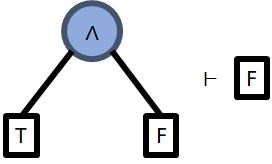
\includegraphics{02_LogicConstructions/Pictures/WedgeEntailment.png}
\end{center}

That gives us a symbolic and visual program to look at commutativity.

\begin{center}
    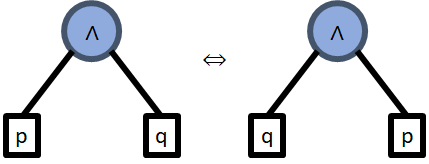
\includegraphics{02_LogicConstructions/Pictures/WedgeCommutativity.png}
\end{center}

\begin{exercise}
We leave it as an exercise to you to determine if XOR is commutative and whether or not implication is commutative. It is recommended that you do this exercise, because the results will be used elsewhere in the book.
\end{exercise}

\subsubsection{Associativity}
Another important property for us to discuss is that of associativity. Whereas commutativity was focused on whether or not we could swap the inputs, associativity is focused on whether we can swap which order we perform actions in.
\begin{samepage}
Starting with the visual programming metaphor, we are interested in knowing whether or not:

\begin{center}
    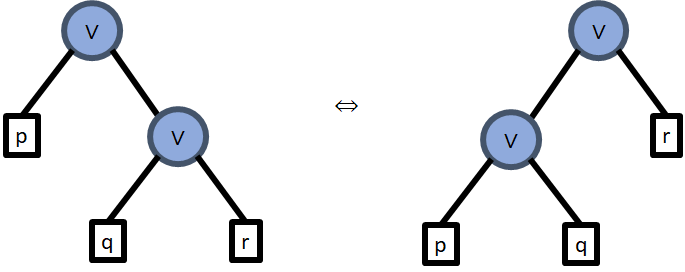
\includegraphics[scale=0.75]{BooleanLogic/Pictures/VeeAssociativity}
\end{center}
\end{samepage}

In order to put this into symbolic form, we use parentheses and brackets to indicate that we want what is inside the parentheses to be computed before everything else. Therefore, we are interested in symbolic form, whether or not:

$$
    (a \vee b) \vee c \iff a \vee (b \vee c)
$$

So, let's start with our proof by exhaustion. We could easily use the Cayley table-type to check commutativity easily, but in this case, associativity is checked best by a Truth-Table:

\begin{table}[ht]
\centering
\begin{tabular}{|c|c|c|c|c|c|c|}
\hline
p & q & r & $p \vee q$ & $q \vee r$ & $p \vee (q \vee r)$ & $(p \vee q) \vee r$ \\ \hline
F & F & F & F       & F       & F               & F               \\ \hline
F & F & T & F       & T       & T               & T               \\ \hline
F & T & F & T       & F       & T               & T               \\ \hline
F & T & T & T       & T       & T               & T               \\ \hline
T & F & F & T       & T       & T               & T               \\ \hline
T & F & T & T       & T       & T               & T               \\ \hline
T & T & F & T       & T       & T               & T               \\ \hline
T & T & T & T       & T       & T               & T               \\ \hline
\end{tabular}
\end{table}

Then, we compare the 2 final columns of the table and see that they are indeed equal.
\begin{samepage}

Since we have proven that, the visual program can be represented even simpler:

\begin{center}
    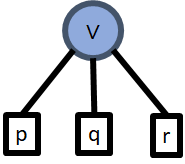
\includegraphics[]{BooleanLogic/Pictures/TotalAssociativity}
\end{center}

Which, symbolically, means that we don't need the parentheses anymore: $a \vee b \vee c$.
\end{samepage}

\begin{exercise}
As a thought-experiment, consider whether or not the idea of commutativity and associativity make sense with Boolean NOT.
\end{exercise}

\begin{exercise}
Now, it is your turn to check that AND, XOR, and implication are associative.
\end{exercise}

\begin{exercise}
Now, you'll notice that when we used tables with 1 Boolean input (NOT), we needed 2 values to describe it. When we used tables to describe operations of 2 values, we needed to compare 4 different combinations (FF, TF, FT, TT) to describe it. Now, describing 3 Boolean inputs, we require 8. Consider what would happen if we had to compare 4 Boolean inputs. Do you see a pattern forming? How many would you need for 5 Boolean inputs?
\end{exercise}

\begin{exercise}
This may serve to be a difficult exercise, but it's worth it. There are actually 2 possible operations that you can perform on 1 Boolean Operation (NOT and ``leave it alone''). With 2 inputs, there are 16 possible Boolean Operations. Using a truth table, find all 16.
\end{exercise}

\begin{exercise}
Using AND, OR, and NOT, you can define XOR like $a \veebar b \iff (a \vee b) \wedge \neg (a \wedge b)$. Use this knowledge to define implication as well.
\end{exercise}

\begin{exercise}
This exercise is not hard, but tedious: Using only implication and the value F (for false), define all 16 of the 2-input Boolean operations.
\end{exercise}

\begin{exercise}
 There is one operation called NOR, which is defined to be the same as $\neg (a \vee b)$. We can symbolically represent this as $a \overline{\vee} b$. With this ONE operation, we can combine it to define implication: $a \implies b \iff ((a \overline{\vee} a) \overline{\vee} b$. In fact, all 16 operations of 2 inputs can be defined with different combinations of NOR. Describe all 16 operations using NOR.
\end{exercise}

\begin{exercise}
Moving on from the previous exercise, find the 1 other operation that has the same property as NOR, such that you can define all 16 operations using it. This and NOR are often used as logic gates in computers.
\end{exercise}

\section{Additional Interpretations of a 2-Value Domain}
The next interpretation is not unique to the Boolean Domain, but can be said of any domain of 2 possible values. The 2 possible values can serve to give us a meaning using future actions.

For instance, we may have the following sentence:
\begin{displayquote}
If Sharon has her truck, she will drive her brother to school; otherwise, Sam will take the bus.
\end{displayquote}

In this situation, we have 2 outcomes, and one \gls{proposition}. A proposition is a statement that can have a truth-value. In our case, we are still working within the Boolean Domain, and so, we assume that our proposition will either be \emph{true} or \emph{false}.

Let's break down the statements and then assign them variables, so that we can get more specific about what we mean:

\begin{samepage}
\begin{itemize}
    \item $t \defeq \textsf{``Sharon has the truck''}$
    \item $r \defeq \textsf{``Sam rides with Sharon to school''}$
    \item $b \defeq \textsf{``Sam takes the bus to school''}$
\end{itemize}
\end{samepage}

In this situation, we have that, if `t' is true, then `r' will happen; otherwise `b' will happen.

Symbolically, we can say that `t' acts on both `r' and `b':

$$
    t\ r\ b
$$
\begin{samepage}

If we define a symbol ($\vdash$), which means, that which is on the left, gives us what is on the right, then we get 2 possible conclusions.

When `t' is true: $T\ r\ b\ \vdash r$

When `t' is false: $F\ r\ b\ \vdash b$

\end{samepage}

Again, many of us do these things in our head so comfortably during everyday conversation that spelling it out like this almost seems unnatural. However, you'll notice that there is a small similarity between our syllogism from logic, in that, if we know the input, we can get the output. In effect, this is what a program does, taking inputs, and computing the output based on the input.

As mentioned in the philosophical discussion, we can consider this like a path, where if we:
\begin{itemize}
    \item have a path start
    \item know where the path leads
\end{itemize}

Then we can conclude that we can get to the destination.

\subsection{Comparing Boolean Logic with 2-Value Interpretation}
If we consider that implication has the meaning that $t \implies r$ means that ``If Sharon has the truck, then she will drive her brother to school'', then our entire sentence actually looks like:

$$
    (t \implies r) \wedge (\neg\ t \implies b)
$$

Giving us the two possible values of `t' ($t$ and $\neg t$), and what each implies.

However, if we do not have a fallback, such as the sentence ``If Keith has \$2, then he'll get chicken nuggets'', we don't have an \emph{otherwise} case. However, we actually do. We have the concept of \emph{no action taken}. In our sentences, this is implicit, but if we are to discuss programs, we may have 2 actions, and the second case may not do anything.

In essence, there is always a second case, even when it's implicit.
\section{Formal Definitions of AND and OR}
We kind of skipped a step in defining AND and OR earlier. This was because it seems obvious to you that AND and OR, as part of our language, must exist with the properties that it has. However, we started with the idea of implication ($a \implies b$) having the same meaning as being ``no more than'' or ``at most'' ($a \leq b$).

We want to understand AND and OR in a similar manner. The best means of doing this is understanding that AND is defined as the truest element `z' that makes $z \leq a$ and $z \leq b$. It can almost be said to pick the minimum truth value between the two, but that can lead us into trouble later. So, if either is `F' then AND must give us `F'. Only when both are `T' can we get `T' as a result.

We also define OR in a similar way, find the smallest truth-value of `z' where $a \leq z$ and $b \leq z$.

\section{Putting Boolean's to Practical Use}
Remember earlier when we said that a single element of a Boolean Domain ($\mathbb{B}$ is called a bit? Having heard that term with regards to computers, it would be a great time to introduce how bits and Boolean Logic are used in computers.

As stated above, a bit can encode the idea of \emph{allow} and \emph{disallow}. Imagine a plastic trough with water. In that trough, there are 2 cutouts below, each that allows for a piece of plastic, the size of the whole, to pass into and stop the flow of water. 

From this, you have constructed a NAND gate if you use water pressure from below to push the plastic pieces up and block the flow of water through the trough. Only if there is no pressure, and both plastic pieces are allowed to fall and barely cover the holes to keep the water from falling out of the trough, water can otherwise flow freely through. That means, pressure applied from below is interpreted as a 1 (T), and no pressure is interpreted as a 0 (F). The result from this is that water can flow freely, interpreted as a 1 (T), or water cannot flow, interpreted as a 0 (F).

\begin{exercise}
Create this water NAND gate out of plastic and/or acrylic, with supervision, if needed.
\end{exercise}

\begin{exercise}
Create an XOR gate using your results from the above exercise, where you found that NAND can be used to create any gate. It may help to use the tree-like diagrams from earlier to do this.
\end{exercise}
\todo{link the exercise, by index to this exercise}

If you have done this, then you can begin to understand how computers work, moving electricity around in a way that is analogous to the water moves through the plastic.

Now, we've left some complexity out in our computer design. For now, to explain the complexity that we will eventually introduce, here is what makes computers work: memory. A small representation of this can be seen here:

\begin{center}
    \makebox[\textwidth]{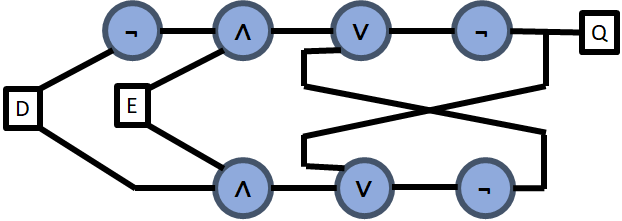
\includegraphics[width=\textwidth]{02_LogicConstructions/Pictures/dFlipFlop.png}}
\end{center}

Reading left-to-right this time, with the inputs on the left, and the outputs on the right, this is called a D register (`D' is for ``direct''), and Q will hold the last value while E is 0. When E is 1, then it gets the value D. You'll notice towards the end (near the right-hand side), some of the output wraps back into more of the circuit. This is called \emph{feedback}, and gives the system memory, enough to hold the value when E is 0.

We won't be working with this at the moment, but it's enough to introduce it, so that you can see how computers begin to be built up from these small gates.

\subsection{8 Bits Make a Byte}
You may have heard that a byte is 8 bits, and if you have, you may have been wondering what importance that even has. Well, we haven't introduced numbers yet in this manual, and I'm going to begin introducing numbers now.

But before I do, I have to introduce several other things. First, is an ordered list, which is nothing more than symbols that are placed in a particular order. As we've said before, mathematicians have various meanings of equality, and in this sense, we are going to define equality on the ordered list $(0, 1)$ to be different from $(1, 0)$. In other words, the order, that the elements are found in, matter.

When we string them together as 01100110 in binary, we are using what is called \gls{PositionalNotation}. The word binary here means only that we have 2 values to work from (our Boolean Domain). As we count, in binary, when we run out of values to increase, we start over, and increase the value on the left of it. It effectively looks like a old-style odometer with only values 0 and 1 for each position:

\todo{find an odometer picture}

\begin{samepage}

Effectively, as we count:
\begin{enumerate}
    \setcounter{enumi}{-1}
    \item 0
    \item 1
    \item 10
    \item 11
    \item 100
    \item 101
    \item 110
    \item 111
    \item 1000
    \item 1001
\end{enumerate}

In this example, I have counted to 9. We could theoretically count forever, always increasing the number of digits in each example.
\end{samepage}

Earlier, you determined that, if you were doing a proof for 2 inputs, you'd need a table using 4 possible values for both inputs. If you did the exercises, and you figured out how to keep going to 3 inputs, or 4 inputs, then you know how many possible values you can get with 8 inputs: 256 possible values.

This means that, 8 bits lets us encode any number from 0 to 255 (we'd lose the ability to encode 256 if we encode 0).

\subsection{Addition}
Starting with small values, we're interested in how to do addition with multiple bits. For that, we need an adder. You should already see that if we have 2 inputs (a and b) and 2 outputs (the topmost digit and the least significant digit), it gives us the following truth table for ($a + b$):

\begin{table}[ht]
\centering
\begin{tabular}{|c|c|c|c||c|c|c|}
a & b & r1 & r0 & $a\wedge b$ & $a \veebar b$ & $a + b$  \\ \hline
0 & 0 & 0 & 0 & 0 & 0 & 00 \\
0 & 1 & 0 & 1 & 0 & 1 & 01 \\
1 & 0 & 0 & 1 & 0 & 1 & 01 \\
1 & 1 & 1 & 0 & 1 & 0 & 10 
\end{tabular}
\end{table}

And you can see that the first digit is $a \veebar b$ and that the second digit is $a \wedge b$.

However, if we are going to make this work for even bigger addition, we need to be able to handle carrying another bit.

\todo{Full adder + adding together with carry.}

\begin{center}
    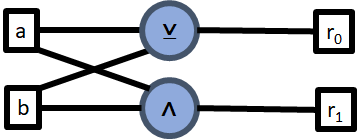
\includegraphics{02_LogicConstructions/Pictures/FullAdder.png}
\end{center}

This is further demonstrating how computers begin to perform more complicated calculations.




\section{Getting Your First Category}
\todo{fill this out}
\section{Applying Logic to Computers}
\todo{fill this out}

\begin{section}{Definitions and Usages of the word Boolean}
    \begin{definition}{Boolean Domain}
        A set with 2 values
    \end{definition}
    \begin{definition}{Boolean Algebra}
    
    \end{definition}

\end{section}